% Options for packages loaded elsewhere
\PassOptionsToPackage{unicode}{hyperref}
\PassOptionsToPackage{hyphens}{url}
%
\documentclass[
]{article}
\usepackage{amsmath,amssymb}
\usepackage{lmodern}
\usepackage{ifxetex,ifluatex}
\ifnum 0\ifxetex 1\fi\ifluatex 1\fi=0 % if pdftex
  \usepackage[T1]{fontenc}
  \usepackage[utf8]{inputenc}
  \usepackage{textcomp} % provide euro and other symbols
\else % if luatex or xetex
  \usepackage{unicode-math}
  \defaultfontfeatures{Scale=MatchLowercase}
  \defaultfontfeatures[\rmfamily]{Ligatures=TeX,Scale=1}
\fi
% Use upquote if available, for straight quotes in verbatim environments
\IfFileExists{upquote.sty}{\usepackage{upquote}}{}
\IfFileExists{microtype.sty}{% use microtype if available
  \usepackage[]{microtype}
  \UseMicrotypeSet[protrusion]{basicmath} % disable protrusion for tt fonts
}{}
\makeatletter
\@ifundefined{KOMAClassName}{% if non-KOMA class
  \IfFileExists{parskip.sty}{%
    \usepackage{parskip}
  }{% else
    \setlength{\parindent}{0pt}
    \setlength{\parskip}{6pt plus 2pt minus 1pt}}
}{% if KOMA class
  \KOMAoptions{parskip=half}}
\makeatother
\usepackage{xcolor}
\IfFileExists{xurl.sty}{\usepackage{xurl}}{} % add URL line breaks if available
\IfFileExists{bookmark.sty}{\usepackage{bookmark}}{\usepackage{hyperref}}
\hypersetup{
  pdftitle={Taller 312},
  pdfauthor={dgonzalez},
  hidelinks,
  pdfcreator={LaTeX via pandoc}}
\urlstyle{same} % disable monospaced font for URLs
\usepackage[margin=1in]{geometry}
\usepackage{color}
\usepackage{fancyvrb}
\newcommand{\VerbBar}{|}
\newcommand{\VERB}{\Verb[commandchars=\\\{\}]}
\DefineVerbatimEnvironment{Highlighting}{Verbatim}{commandchars=\\\{\}}
% Add ',fontsize=\small' for more characters per line
\usepackage{framed}
\definecolor{shadecolor}{RGB}{248,248,248}
\newenvironment{Shaded}{\begin{snugshade}}{\end{snugshade}}
\newcommand{\AlertTok}[1]{\textcolor[rgb]{0.94,0.16,0.16}{#1}}
\newcommand{\AnnotationTok}[1]{\textcolor[rgb]{0.56,0.35,0.01}{\textbf{\textit{#1}}}}
\newcommand{\AttributeTok}[1]{\textcolor[rgb]{0.77,0.63,0.00}{#1}}
\newcommand{\BaseNTok}[1]{\textcolor[rgb]{0.00,0.00,0.81}{#1}}
\newcommand{\BuiltInTok}[1]{#1}
\newcommand{\CharTok}[1]{\textcolor[rgb]{0.31,0.60,0.02}{#1}}
\newcommand{\CommentTok}[1]{\textcolor[rgb]{0.56,0.35,0.01}{\textit{#1}}}
\newcommand{\CommentVarTok}[1]{\textcolor[rgb]{0.56,0.35,0.01}{\textbf{\textit{#1}}}}
\newcommand{\ConstantTok}[1]{\textcolor[rgb]{0.00,0.00,0.00}{#1}}
\newcommand{\ControlFlowTok}[1]{\textcolor[rgb]{0.13,0.29,0.53}{\textbf{#1}}}
\newcommand{\DataTypeTok}[1]{\textcolor[rgb]{0.13,0.29,0.53}{#1}}
\newcommand{\DecValTok}[1]{\textcolor[rgb]{0.00,0.00,0.81}{#1}}
\newcommand{\DocumentationTok}[1]{\textcolor[rgb]{0.56,0.35,0.01}{\textbf{\textit{#1}}}}
\newcommand{\ErrorTok}[1]{\textcolor[rgb]{0.64,0.00,0.00}{\textbf{#1}}}
\newcommand{\ExtensionTok}[1]{#1}
\newcommand{\FloatTok}[1]{\textcolor[rgb]{0.00,0.00,0.81}{#1}}
\newcommand{\FunctionTok}[1]{\textcolor[rgb]{0.00,0.00,0.00}{#1}}
\newcommand{\ImportTok}[1]{#1}
\newcommand{\InformationTok}[1]{\textcolor[rgb]{0.56,0.35,0.01}{\textbf{\textit{#1}}}}
\newcommand{\KeywordTok}[1]{\textcolor[rgb]{0.13,0.29,0.53}{\textbf{#1}}}
\newcommand{\NormalTok}[1]{#1}
\newcommand{\OperatorTok}[1]{\textcolor[rgb]{0.81,0.36,0.00}{\textbf{#1}}}
\newcommand{\OtherTok}[1]{\textcolor[rgb]{0.56,0.35,0.01}{#1}}
\newcommand{\PreprocessorTok}[1]{\textcolor[rgb]{0.56,0.35,0.01}{\textit{#1}}}
\newcommand{\RegionMarkerTok}[1]{#1}
\newcommand{\SpecialCharTok}[1]{\textcolor[rgb]{0.00,0.00,0.00}{#1}}
\newcommand{\SpecialStringTok}[1]{\textcolor[rgb]{0.31,0.60,0.02}{#1}}
\newcommand{\StringTok}[1]{\textcolor[rgb]{0.31,0.60,0.02}{#1}}
\newcommand{\VariableTok}[1]{\textcolor[rgb]{0.00,0.00,0.00}{#1}}
\newcommand{\VerbatimStringTok}[1]{\textcolor[rgb]{0.31,0.60,0.02}{#1}}
\newcommand{\WarningTok}[1]{\textcolor[rgb]{0.56,0.35,0.01}{\textbf{\textit{#1}}}}
\usepackage{graphicx}
\makeatletter
\def\maxwidth{\ifdim\Gin@nat@width>\linewidth\linewidth\else\Gin@nat@width\fi}
\def\maxheight{\ifdim\Gin@nat@height>\textheight\textheight\else\Gin@nat@height\fi}
\makeatother
% Scale images if necessary, so that they will not overflow the page
% margins by default, and it is still possible to overwrite the defaults
% using explicit options in \includegraphics[width, height, ...]{}
\setkeys{Gin}{width=\maxwidth,height=\maxheight,keepaspectratio}
% Set default figure placement to htbp
\makeatletter
\def\fps@figure{htbp}
\makeatother
\setlength{\emergencystretch}{3em} % prevent overfull lines
\providecommand{\tightlist}{%
  \setlength{\itemsep}{0pt}\setlength{\parskip}{0pt}}
\setcounter{secnumdepth}{-\maxdimen} % remove section numbering
\ifluatex
  \usepackage{selnolig}  % disable illegal ligatures
\fi

\title{Taller 312}
\usepackage{etoolbox}
\makeatletter
\providecommand{\subtitle}[1]{% add subtitle to \maketitle
  \apptocmd{\@title}{\par {\large #1 \par}}{}{}
}
\makeatother
\subtitle{Taller 302}
\author{dgonzalez}
\date{}

\begin{document}
\maketitle

{
\setcounter{tocdepth}{2}
\tableofcontents
}
\hypertarget{punto-1}{%
\subsection{Punto 1}\label{punto-1}}

Suponga que \(f_X(x)=exp(-x)\) para \(0<x\) , \(0\) en cualquier otro
caso. Determine:

\begin{Shaded}
\begin{Highlighting}[]
\NormalTok{fx1}\OtherTok{=}\ControlFlowTok{function}\NormalTok{(x)\{}\FunctionTok{exp}\NormalTok{(}\SpecialCharTok{{-}}\NormalTok{x)\}}
\NormalTok{x1}\OtherTok{=}\FunctionTok{seq}\NormalTok{(}\DecValTok{0}\NormalTok{,}\DecValTok{5}\NormalTok{,}\FloatTok{0.1}\NormalTok{)}
\NormalTok{fx}\OtherTok{=}\FunctionTok{fx1}\NormalTok{(x1)}
\FunctionTok{plot}\NormalTok{(x1,fx, }\AttributeTok{type=}\StringTok{"l"}\NormalTok{)}
\FunctionTok{grid}\NormalTok{()}
\end{Highlighting}
\end{Shaded}

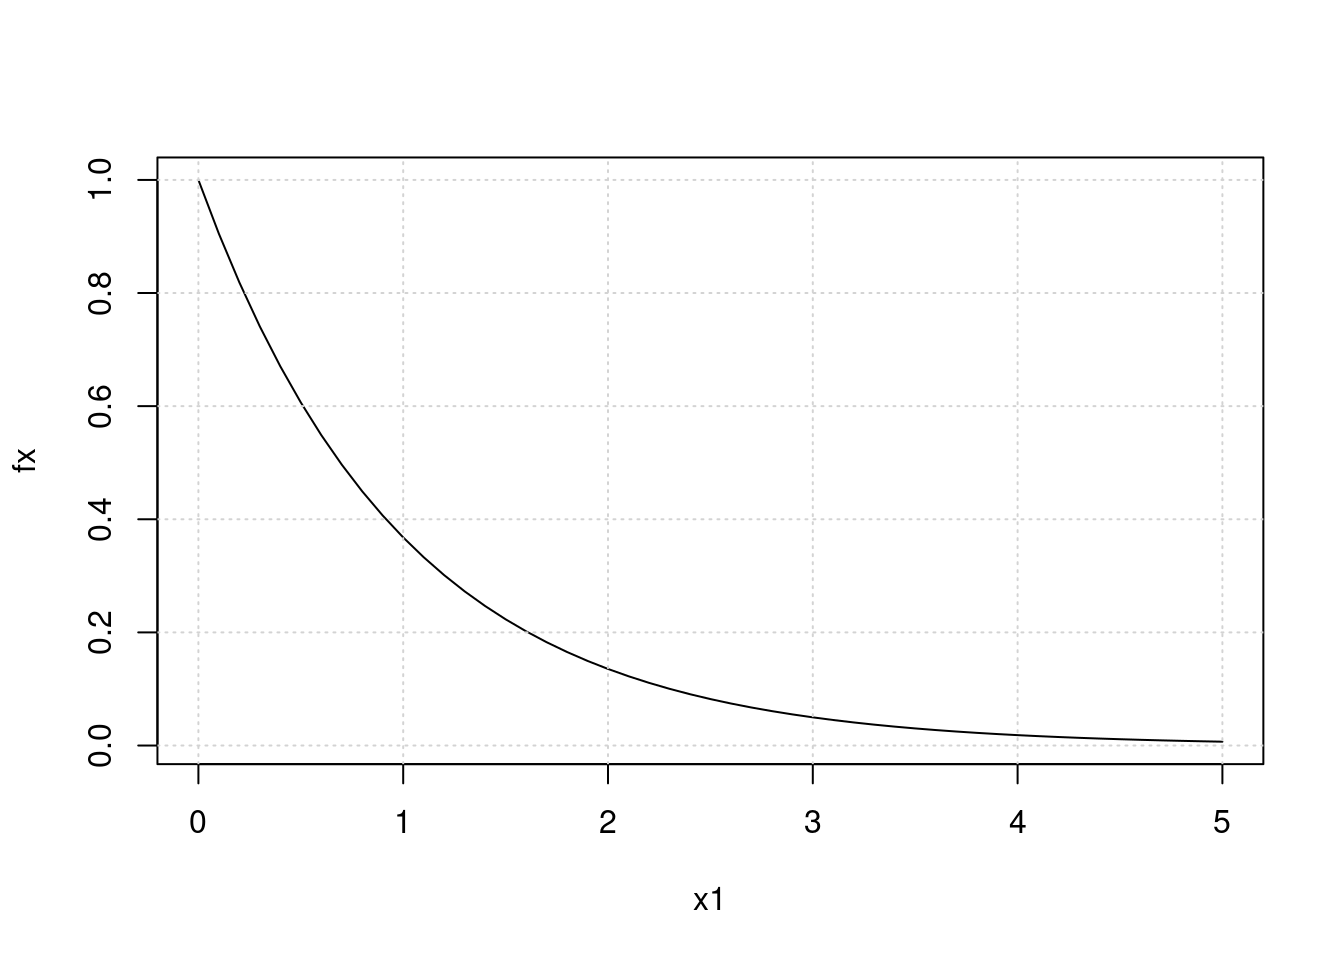
\includegraphics{Taller312_files/figure-latex/unnamed-chunk-1-1.pdf}

\begin{Shaded}
\begin{Highlighting}[]
\NormalTok{x}\OtherTok{=}\FunctionTok{seq}\NormalTok{(}\DecValTok{0}\NormalTok{,}\DecValTok{5}\NormalTok{, }\AttributeTok{by=}\FloatTok{0.1}\NormalTok{)}
\NormalTok{fx}\OtherTok{=}\FunctionTok{fx1}\NormalTok{(x)}

\NormalTok{x}\FloatTok{.1}\OtherTok{=}\FunctionTok{c}\NormalTok{(}\DecValTok{0}\NormalTok{,x,}\DecValTok{5}\NormalTok{)}
\NormalTok{fx}\FloatTok{.1}\OtherTok{=}\FunctionTok{c}\NormalTok{(}\DecValTok{0}\NormalTok{,fx,}\DecValTok{0}\NormalTok{)}

\FunctionTok{plot}\NormalTok{(x,fx, }\AttributeTok{type=}\StringTok{"l"}\NormalTok{, }\AttributeTok{ylim=}\FunctionTok{c}\NormalTok{(}\DecValTok{0}\NormalTok{,}\DecValTok{1}\NormalTok{),}\AttributeTok{col=}\StringTok{"blue"}\NormalTok{, }\AttributeTok{lwd=}\DecValTok{5}\NormalTok{, }\AttributeTok{xlim=}\FunctionTok{c}\NormalTok{(}\DecValTok{0}\NormalTok{,}\DecValTok{5}\NormalTok{)) }\CommentTok{\# forma 2}
\FunctionTok{polygon}\NormalTok{(x}\FloatTok{.1}\NormalTok{,fx}\FloatTok{.1}\NormalTok{,}\AttributeTok{col =} \StringTok{"\#1b98e0"}\NormalTok{) }
\end{Highlighting}
\end{Shaded}

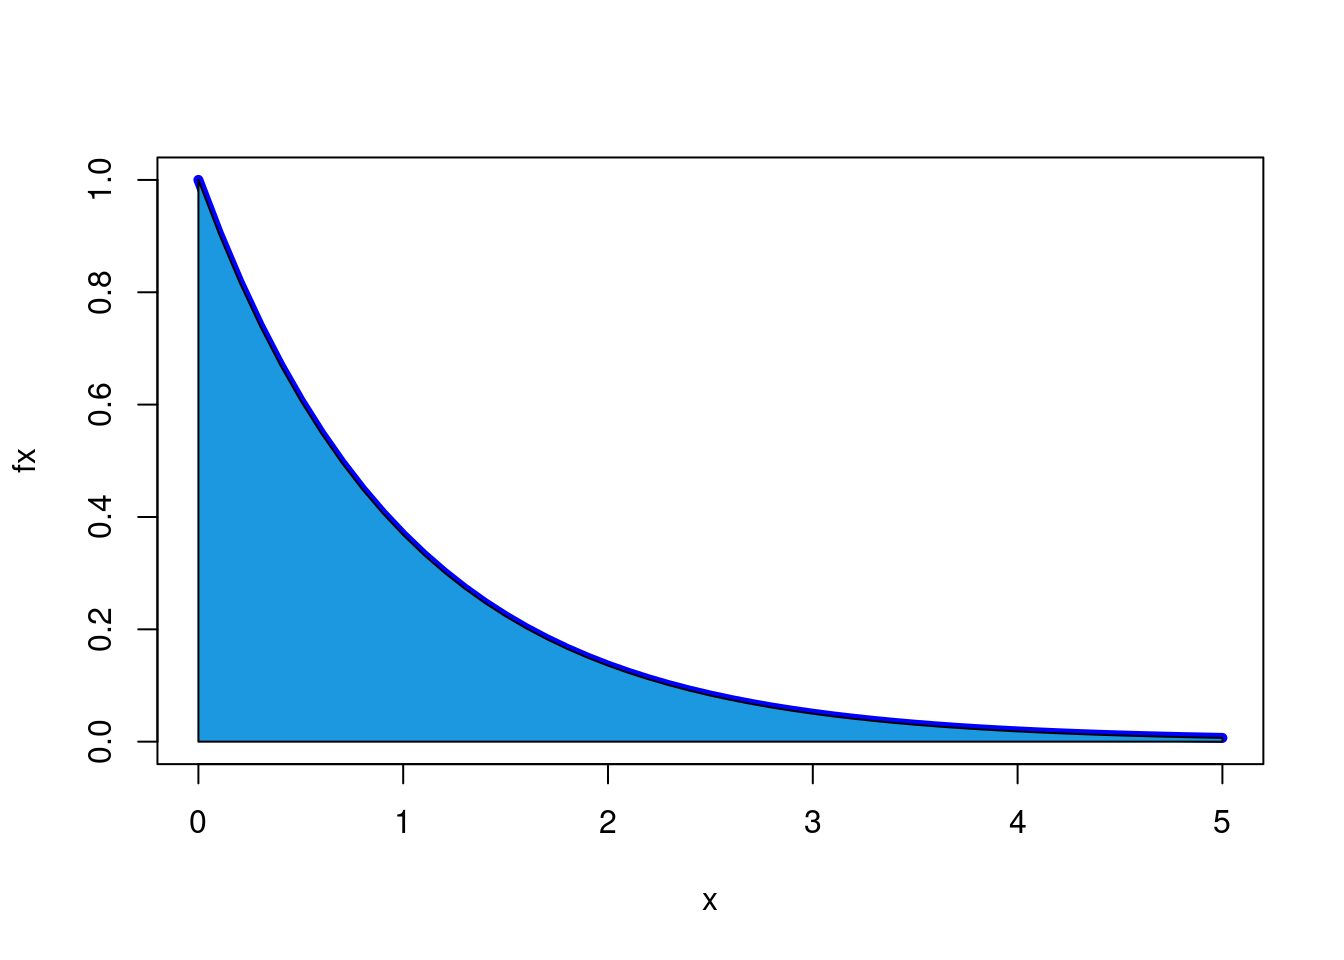
\includegraphics{Taller312_files/figure-latex/unnamed-chunk-1-2.pdf}

\begin{Shaded}
\begin{Highlighting}[]
\FunctionTok{integrate}\NormalTok{(fx1,}\DecValTok{0}\NormalTok{,}\ConstantTok{Inf}\NormalTok{) }\CommentTok{\# verificacion de que f(x) es una funcion de densidad de probabilidad}
\end{Highlighting}
\end{Shaded}

\begin{verbatim}
## 1 with absolute error < 5.7e-05
\end{verbatim}

\begin{itemize}
\tightlist
\item
  \(P(1 < X)\)
\end{itemize}

\begin{Shaded}
\begin{Highlighting}[]
\NormalTok{x}\OtherTok{=}\FunctionTok{seq}\NormalTok{(}\DecValTok{1}\NormalTok{,}\DecValTok{5}\NormalTok{, }\AttributeTok{by=}\FloatTok{0.1}\NormalTok{)}
\NormalTok{fx}\OtherTok{=}\FunctionTok{fx1}\NormalTok{(x)}

\NormalTok{x}\FloatTok{.1}\NormalTok{a}\OtherTok{=}\FunctionTok{c}\NormalTok{(}\DecValTok{1}\NormalTok{,x,}\DecValTok{5}\NormalTok{)}
\NormalTok{fx}\FloatTok{.1}\NormalTok{a}\OtherTok{=}\FunctionTok{c}\NormalTok{(}\DecValTok{0}\NormalTok{,fx,}\DecValTok{0}\NormalTok{)}

\FunctionTok{plot}\NormalTok{(x,fx, }\AttributeTok{type=}\StringTok{"l"}\NormalTok{, }\AttributeTok{ylim=}\FunctionTok{c}\NormalTok{(}\DecValTok{0}\NormalTok{,}\DecValTok{1}\NormalTok{),}\AttributeTok{col=}\StringTok{"blue"}\NormalTok{, }\AttributeTok{lwd=}\DecValTok{5}\NormalTok{, }\AttributeTok{xlim=}\FunctionTok{c}\NormalTok{(}\DecValTok{0}\NormalTok{,}\DecValTok{5}\NormalTok{)) }\CommentTok{\# forma 2}
\FunctionTok{polygon}\NormalTok{(x}\FloatTok{.1}\NormalTok{a,fx}\FloatTok{.1}\NormalTok{a,}\AttributeTok{col =} \StringTok{"\#1b98e0"}\NormalTok{) }
\end{Highlighting}
\end{Shaded}

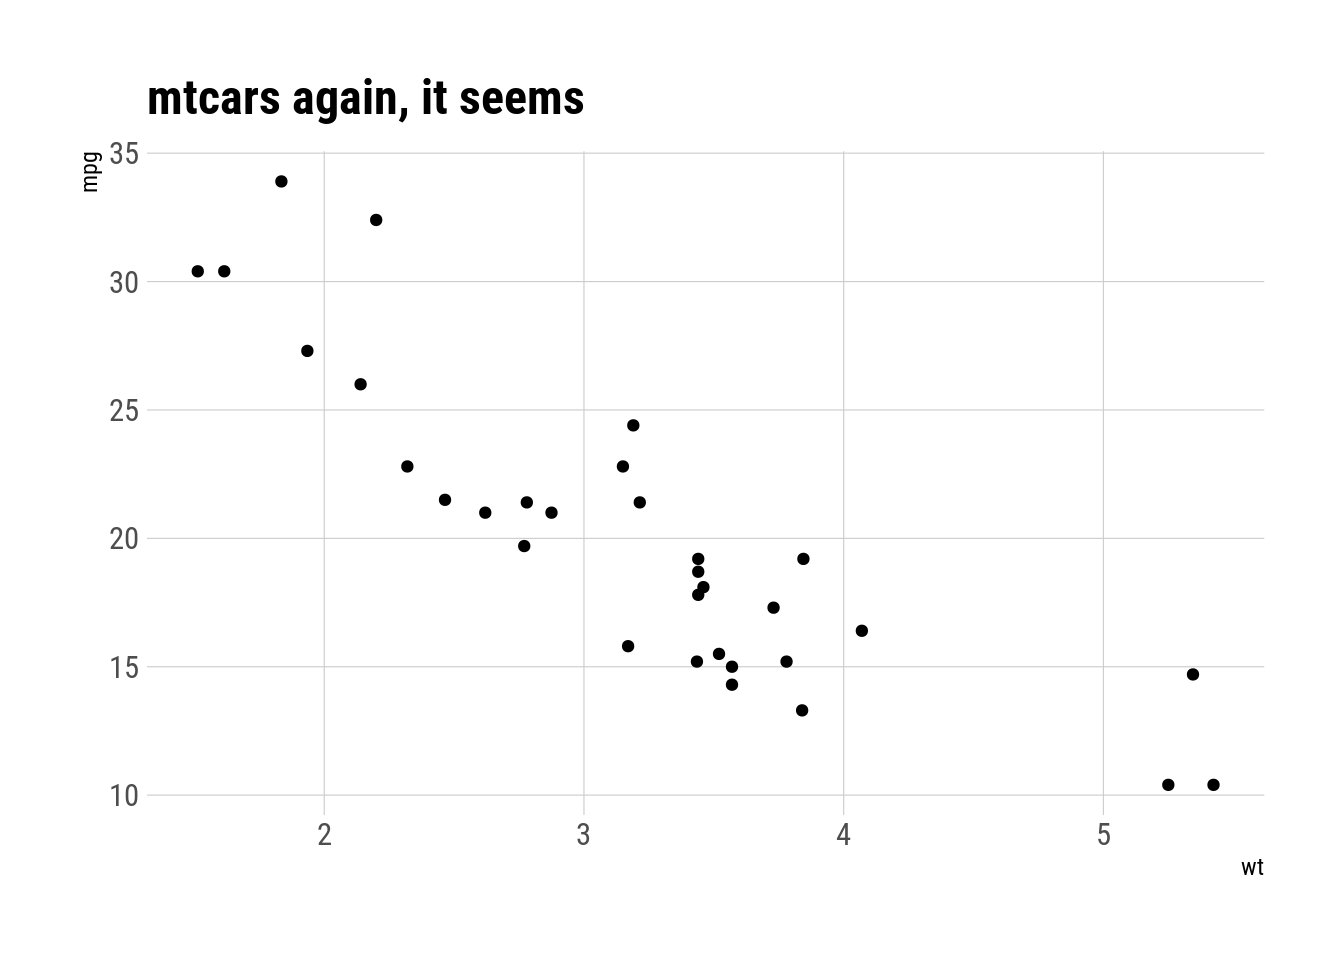
\includegraphics{Taller312_files/figure-latex/unnamed-chunk-2-1.pdf}

\begin{Shaded}
\begin{Highlighting}[]
\FunctionTok{integrate}\NormalTok{(fx1,}\DecValTok{1}\NormalTok{,}\ConstantTok{Inf}\NormalTok{) }\CommentTok{\# P(X\textgreater{}1)}
\end{Highlighting}
\end{Shaded}

\begin{verbatim}
## 0.3678794 with absolute error < 2.1e-05
\end{verbatim}

\begin{itemize}
\item
  \(P(1 < X < 2.5)\)
\item
  \(P(X = 3)\)
\item
  \(P(X<4)\)
\item
  \(Me\)
\item
  \(Q_{1}\)
\item
  \(Q_{3}\)
\item
  \(E[X]\)
\end{itemize}

\begin{Shaded}
\begin{Highlighting}[]
\NormalTok{fxx}\OtherTok{=}\ControlFlowTok{function}\NormalTok{(x)\{x}\SpecialCharTok{*}\FunctionTok{exp}\NormalTok{(}\SpecialCharTok{{-}}\NormalTok{x)\}}
\FunctionTok{integrate}\NormalTok{(fxx,}\DecValTok{0}\NormalTok{,}\ConstantTok{Inf}\NormalTok{)}
\end{Highlighting}
\end{Shaded}

\begin{verbatim}
## 1 with absolute error < 6.4e-06
\end{verbatim}

\begin{itemize}
\tightlist
\item
  \(V[X]\)
\end{itemize}

\begin{Shaded}
\begin{Highlighting}[]
\NormalTok{fxx}\OtherTok{=}\ControlFlowTok{function}\NormalTok{(x)\{x}\SpecialCharTok{*}\FunctionTok{exp}\NormalTok{(}\SpecialCharTok{{-}}\NormalTok{x)\}}
\NormalTok{Ex}\OtherTok{=}\FunctionTok{integrate}\NormalTok{(fxx,}\DecValTok{0}\NormalTok{,}\ConstantTok{Inf}\NormalTok{)  }\CommentTok{\# valor esperado de X. primer momento}

\NormalTok{fxx}\OtherTok{=}\ControlFlowTok{function}\NormalTok{(x)\{x}\SpecialCharTok{\^{}}\DecValTok{2}\SpecialCharTok{*}\FunctionTok{exp}\NormalTok{(}\SpecialCharTok{{-}}\NormalTok{x)\}}
\NormalTok{Ex2}\OtherTok{=}\FunctionTok{integrate}\NormalTok{(fxx,}\DecValTok{0}\NormalTok{,}\ConstantTok{Inf}\NormalTok{)  }\CommentTok{\# segundo momento  de X}

\NormalTok{Vx}\OtherTok{=}\NormalTok{Ex2}\SpecialCharTok{$}\NormalTok{value}\SpecialCharTok{{-}}\NormalTok{Ex}\SpecialCharTok{$}\NormalTok{value}\SpecialCharTok{\^{}}\DecValTok{2} \CommentTok{\# varianza de X}
\NormalTok{Vx }
\end{Highlighting}
\end{Shaded}

\begin{verbatim}
## [1] 1
\end{verbatim}

\hypertarget{punto-2}{%
\subsection{Punto 2}\label{punto-2}}

Suponga que X es una variable aleatoria continua con funcio de
distribucion acumulada

\[f(x)=\left\{\begin{matrix}0&\mbox{si }x<0\\ 2x & \mbox{si } 0 < x < 5 \\ 
                      1  & \mbox{si } 5 \leq x  \end{matrix}\right. \]

\begin{itemize}
\item
  \(P(X < 2)\)
\item
  \(P(X = 1.5)\)
\item
  \(P( X > 3)\)
\item
  \(P(0.5 < X <2.7)\)
\end{itemize}

\hypertarget{punto-3}{%
\subsection{Punto 3}\label{punto-3}}

Para una variable aleatoria con funcion de distribucion:

\[f(x)=\left\{\begin{matrix}\dfrac{(2x+1)}{25}& x=0,1,2,3,4.\\ & \\
 0 & \mbox{para cualquier otro caso} \end{matrix}\right.\]

\begin{Shaded}
\begin{Highlighting}[]
\NormalTok{fx3}\OtherTok{=}\ControlFlowTok{function}\NormalTok{(x)\{(}\DecValTok{2}\SpecialCharTok{*}\NormalTok{x}\SpecialCharTok{+}\DecValTok{1}\NormalTok{)}\SpecialCharTok{/}\DecValTok{25}\NormalTok{\}}
\NormalTok{x}\OtherTok{=}\DecValTok{0}\SpecialCharTok{:}\DecValTok{4}
\FunctionTok{plot}\NormalTok{(x,}\FunctionTok{fx3}\NormalTok{(x), }\AttributeTok{pch=}\DecValTok{19}\NormalTok{)}
\end{Highlighting}
\end{Shaded}

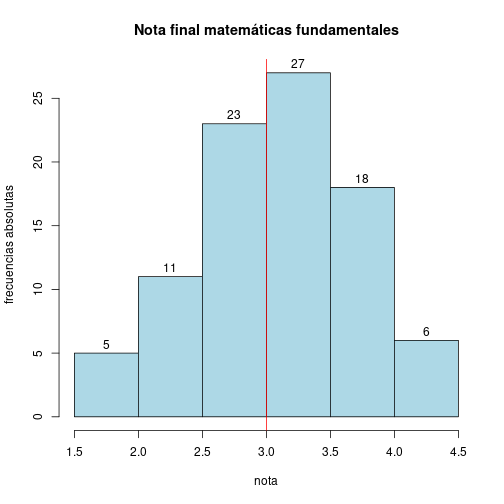
\includegraphics{Taller312_files/figure-latex/unnamed-chunk-5-1.pdf}

\begin{Shaded}
\begin{Highlighting}[]
\FunctionTok{sum}\NormalTok{(}\FunctionTok{fx3}\NormalTok{(x)) }\CommentTok{\# verificacion de que f(x) es una funcion de distribucion de probabilidad}
\end{Highlighting}
\end{Shaded}

\begin{verbatim}
## [1] 1
\end{verbatim}

\begin{itemize}
\item
  \(P(X=4)\)
\item
  \(P(X\leq 1)\)
\item
  P(2 \leq X \textless{} 4)\$
\item
  \(E[X]\)
\item
  \(V[X]\)
\end{itemize}

\hypertarget{punto-4}{%
\subsection{Punto 4}\label{punto-4}}

Para una variable aleatoria con funcion de distribucion de probabilidad
\(f(x)=(3/4)(1/4)^{x}\), para \$x=0,1,2,3,\ldots\ldots. \$

\begin{Shaded}
\begin{Highlighting}[]
\NormalTok{x}\OtherTok{=}\DecValTok{0}\SpecialCharTok{:}\DecValTok{10}
\FunctionTok{plot}\NormalTok{(x,}\FunctionTok{fx4}\NormalTok{(x), }\AttributeTok{pch=}\DecValTok{19}\NormalTok{)}
\end{Highlighting}
\end{Shaded}

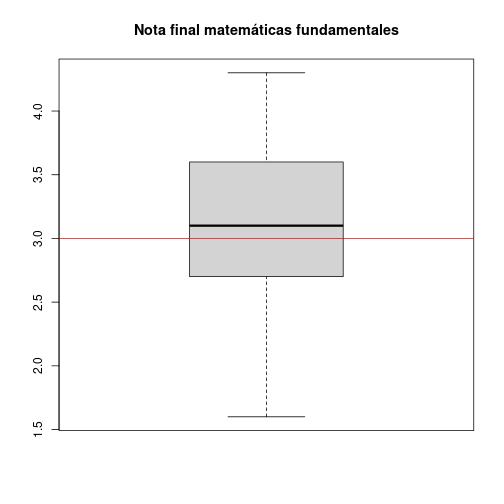
\includegraphics{Taller312_files/figure-latex/unnamed-chunk-6-1.pdf}

\begin{itemize}
\item
  \(P(X=2)\)
\item
  \(P(X\leq 2)\)
\item
  \(P(X < 2)\)
\item
  \(P(X > 2)\)
\item
  \(E[X]\)
\item
  \(V[X]\)
\end{itemize}

\hypertarget{punto-13}{%
\subsection{Punto 13}\label{punto-13}}

\[\binom{25}{x}0.80^x 0.20^{25-x}\]

\begin{Shaded}
\begin{Highlighting}[]
\NormalTok{fx}\OtherTok{=}\ControlFlowTok{function}\NormalTok{(x)\{}\FunctionTok{choose}\NormalTok{(}\DecValTok{25}\NormalTok{,x)}\SpecialCharTok{*}\FloatTok{0.80}\SpecialCharTok{\^{}}\NormalTok{x}\SpecialCharTok{*}\NormalTok{(}\DecValTok{1}\FloatTok{{-}0.80}\NormalTok{)}\SpecialCharTok{\^{}}\NormalTok{(}\DecValTok{25}\SpecialCharTok{{-}}\NormalTok{x)\}}
\NormalTok{x}\OtherTok{=}\DecValTok{0}\SpecialCharTok{:}\DecValTok{25}
\NormalTok{f.x}\OtherTok{=}\FunctionTok{fx}\NormalTok{(x)}
\FunctionTok{plot}\NormalTok{(x,f.x, }\AttributeTok{pch=}\DecValTok{19}\NormalTok{)}
\end{Highlighting}
\end{Shaded}

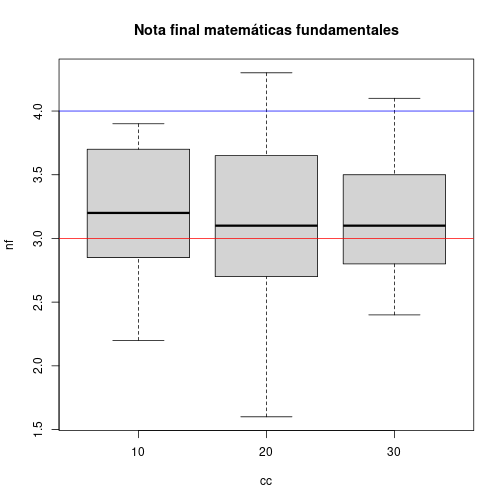
\includegraphics{Taller312_files/figure-latex/unnamed-chunk-7-1.pdf}

\begin{Shaded}
\begin{Highlighting}[]
\FunctionTok{sum}\NormalTok{(f.x) }\CommentTok{\# verificacion de que f(x) es una fun.de distribucion de probabilidad}
\end{Highlighting}
\end{Shaded}

\begin{verbatim}
## [1] 1
\end{verbatim}

\begin{Shaded}
\begin{Highlighting}[]
\FunctionTok{fx}\NormalTok{(}\DecValTok{20}\NormalTok{) }\CommentTok{\# P(X=20)}
\end{Highlighting}
\end{Shaded}

\begin{verbatim}
## [1] 0.1960151
\end{verbatim}

\begin{Shaded}
\begin{Highlighting}[]
\FunctionTok{sum}\NormalTok{(f.x[}\DecValTok{0}\SpecialCharTok{:}\DecValTok{20}\NormalTok{]) }\CommentTok{\# P(X\textless{}=20)}
\end{Highlighting}
\end{Shaded}

\begin{verbatim}
## [1] 0.3833106
\end{verbatim}

\end{document}
